\documentclass[a4,11pt]{aleph-notas}

% -- Paquetes adicionales
\usepackage{enumitem}
\usepackage{aleph-comandos}
\usepackage{systeme}

% -- Datos 
\institucion{Escuela de Ciencias Físicas y Matemática}
\carrera{Bioingeniería}
\asignatura{Álgebra lineal}
\tema{Clase invertida no. 1: Cálculo de determinantes}
\autor[A. Merino]{Andrés Merino}
\fecha{Semestre 2024-1}

\logouno[0.14\textwidth]{Logos/logoPUCE_04_ac}
\definecolor{colortext}{HTML}{0030A1}
\definecolor{colordef}{HTML}{0030A1}
\fuente{montserrat}

% -- Comandos adicionales
\begin{document}

\encabezado

\vspace*{-10mm}
\section*{Introducción}

\begin{itemize}
    \item \textbf{Tema:} Determinantes
    \item \textbf{Resultado de Aprendizaje:} Calcula determinantes de matrices usando menores.
\end{itemize}

\section*{Lección en casa}

\subsection*{Actividades}

\begin{enumerate}[leftmargin=*]
    \item Interactuar con ChatGPT mediante los siguientes \textit{prompts}, leyendo detenidamente el \textit{prompt} y su respuesta:
    \begin{enumerate}[label=\textit{Prompt \arabic*.},leftmargin=2.1cm]
        \item Vas a ser mi profesor de la asignatura de Álgebra Lineal, te iré dando indicaciones y me irás explicando de manera formal y luego de manera intuitiva los conceptos. Vas a tener mucho cuidado al escribir la parte matemática para que se visualice bien. ¿Entendido?
        \item Dada una matriz A, ¿qué es la matriz (i,j)-menor que la llamaremos A\_ij? Dame un ejemplo revisado de manera cuidadosa para A\_11 y A\_12.
        \item ¿Qué es el determinante de una matriz? Quiero solo la idea intuitiva.
        \item ¿Cómo se calcula el determinante de una matriz de 1$\times$1? Dame un ejemplo numérico.
        \item ¿Cómo se calcula el determinante de una matriz de 2$\times$2 usando expansión por menores de la primera fila? Dame un ejemplo numérico.
        \item ¿Cómo se calcula el determinante de una matriz de 3$\times$3 usando expansión por menores de la primera fila? Dame un ejemplo numérico.
        \item Explícame el cálculo del determinante (usando expansión por menores de la primera fila) de la siguiente matriz\\
        1 5 3\\
        -4 8 9\\
        4 2 1
        \item Evalúame para determinar si he comprendido. Escríbeme una pregunta y te daré la respuesta, luego me darás retroalimentación y proseguirás con otra pregunta.
    \end{enumerate}
    \item Continuar la interacción hasta que te sientas preparado en el cálculo de determinantes.
    \item Copiar el enlace del chat como evidencia del proceso (ver Anexo).
    \item En caso de tener dudas sobre el tema, interactúa con tus compañeros de clase para solventarlas.
    \item Realiza el cuestionario del aula virtual.
\end{enumerate}

\section*{Anexo}

\subsection*{¿Cómo obtener el enlace de una conversación con ChatGPT?}

Seguir los siguientes pasos:
\begin{enumerate}
    \item Dar clic en los tres puntos a lado del nombre de la conversación.
    \item Seleccionar «Compartir».
    \begin{center}
        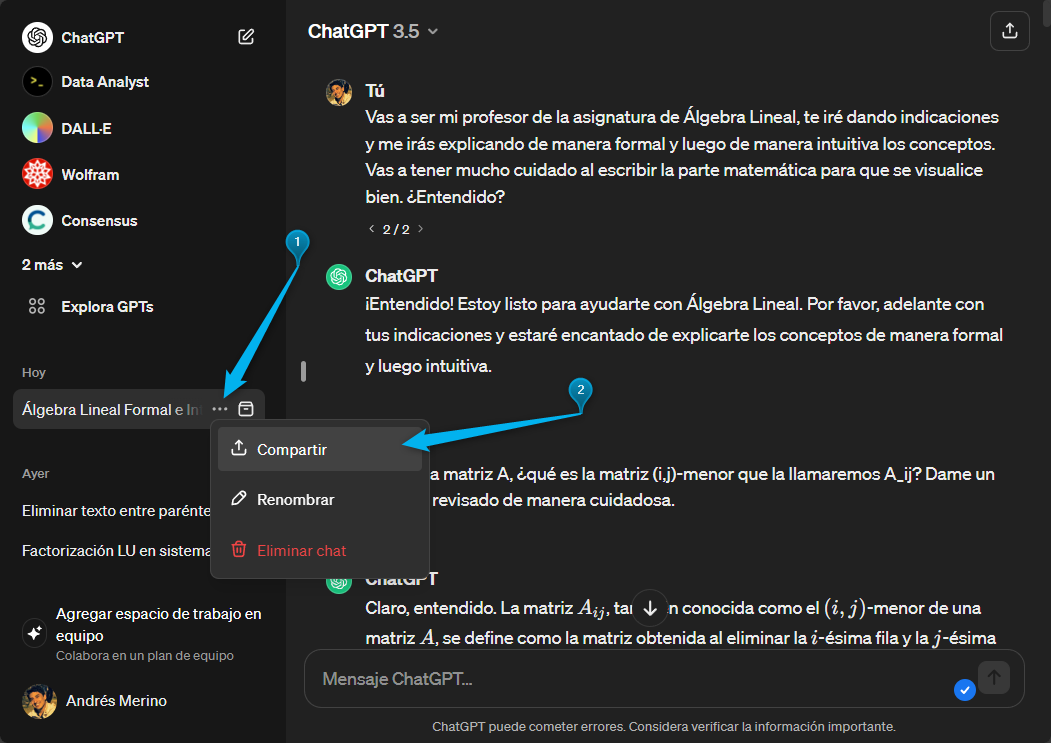
\includegraphics[width=0.85\linewidth]{fig01.png}
    \end{center}
    \item En la nueva ventana, dar clic en los tres puntos. 
    \item Seleccionar «Compartir tu nombre».
    \item Dar clic en «Compartir enlace».

    \begin{center}
        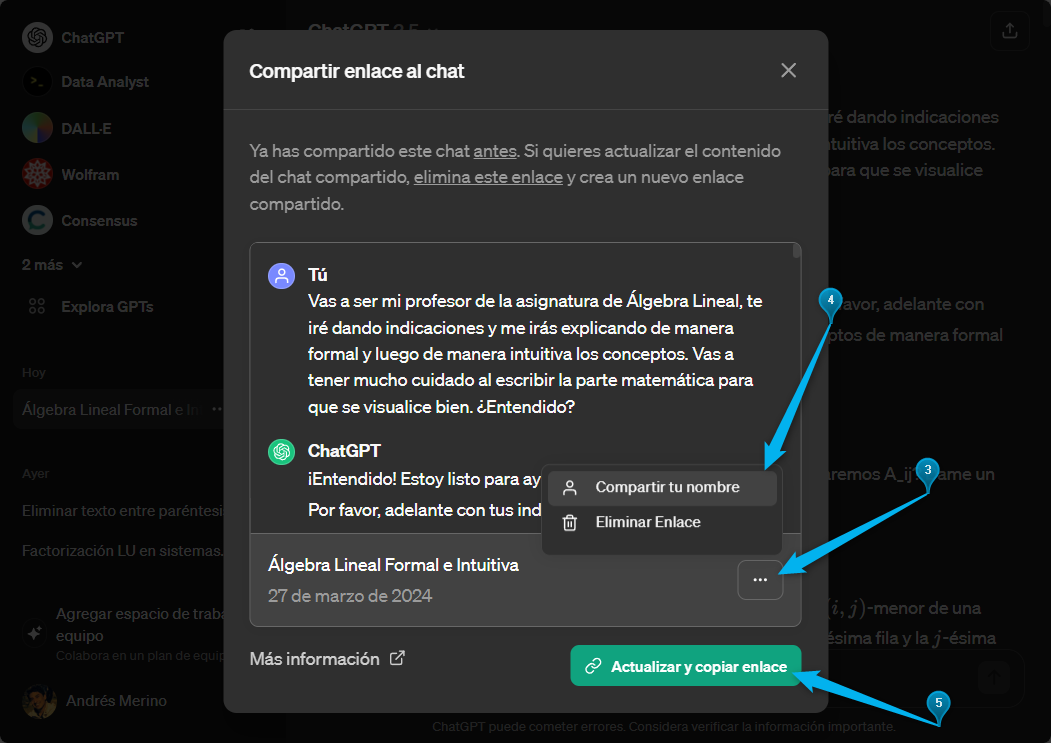
\includegraphics[width=0.85\linewidth]{fig02.png}
    \end{center}
\end{enumerate}


\end{document}